\chapter{THEROTICAL FRAMEWORK}\label{introduction}
\graphicspath{{images/}}

% Importance of ankle in the gait and all the diseases that causes footdrop or similars, and the solutions for this desease.

\section{theoretical framework}\label{framework}

\section{Human gait}

The gait analysis is carried out on the basis of the gait cycle, that can be taken as representation of person's walking patterns, and comparison of several cycles indicates the variability of the pattern \cite{Baker2013}. The gait cycle is normalized from 0\% to 100\%, because each pattern have different timing, so is not objective realize a comparison between them \cite{Medved2021}, it can be described with spatial and temporal parameters. 
% \subsection{Spatial parameters}

% The main spatial parameters are shown in figure \ref{step_stride} and described bellow:

% \begin{itemize}
%     \item Step: the movement of the one foot in front of the other.
%     \item Stride: step of one foot followed by another step for the other. 
%     \item Foot contact: it is considered as the beginning of the gait cycle, in healthy people it is referred to as \textit{heel strike}.  
%     \item Step length: distance traveled for one foot in front of the same part of the other foot.
%     \item Stride length: distance between two consecutive gait cycles.
%     \item Step width: mediolateral separation of the feet, also known as stride width.
% \end{itemize}

% \begin{figure}
%     \centering
%     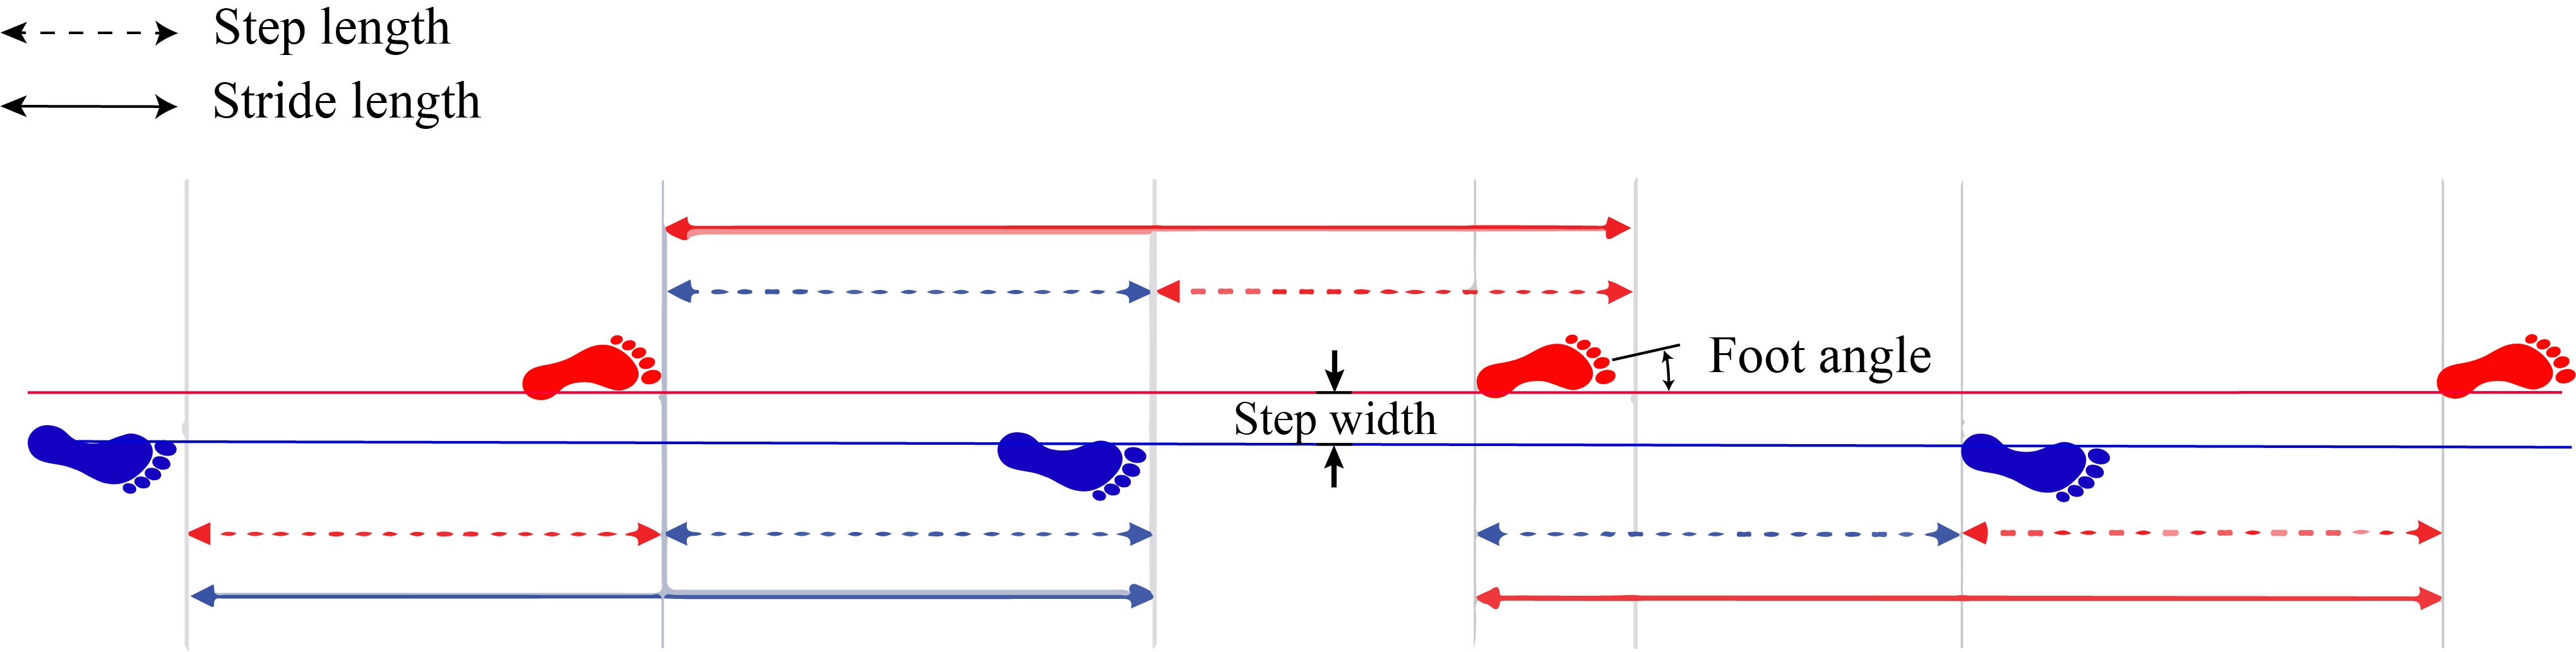
\includegraphics[width=1\textwidth]{step_stride.png}
%     \caption[Gait spatial parameters]{Gait spatial parameters. Source: edited by author from \cite{Baker2013}.}
%     \label{step_stride}
% \end{figure}

% \subsection{Temporal parameters}
% Temporal parameters are listed bellow:

% \begin{itemize}
%     \item Stride time: duration of gait cycle (time between two foot strikes). 
%     \item Cadence: it is a more commonly term used to specify the duration of the cycle in indirect way. And is described by: 
%     \begin{equation}
%         \frac{\#cycles}{time\hspace{1mm}interval}
%     \end{equation}
%     \item Walking speed: distance traveled in a given time in meters/second, if cadence is in steps per minute and stride length is in meters the calculation is given by:
%     \begin{equation}
%         \frac{cadence*stride\hspace{1mm}length}{120}
%     \end{equation}
% \end{itemize}

% Gait is globally divided into two phases, \textit{stance} and \textit{swing}. The first occur when foot is in contact with the ground, on the other hand, the swing occur when it is not. The stance phase ends when foot off (toe off); the same point at which the swing begins, as illustrated in the figure \ref{gait_phases}, 

% \begin{figure}
%     \centering
%     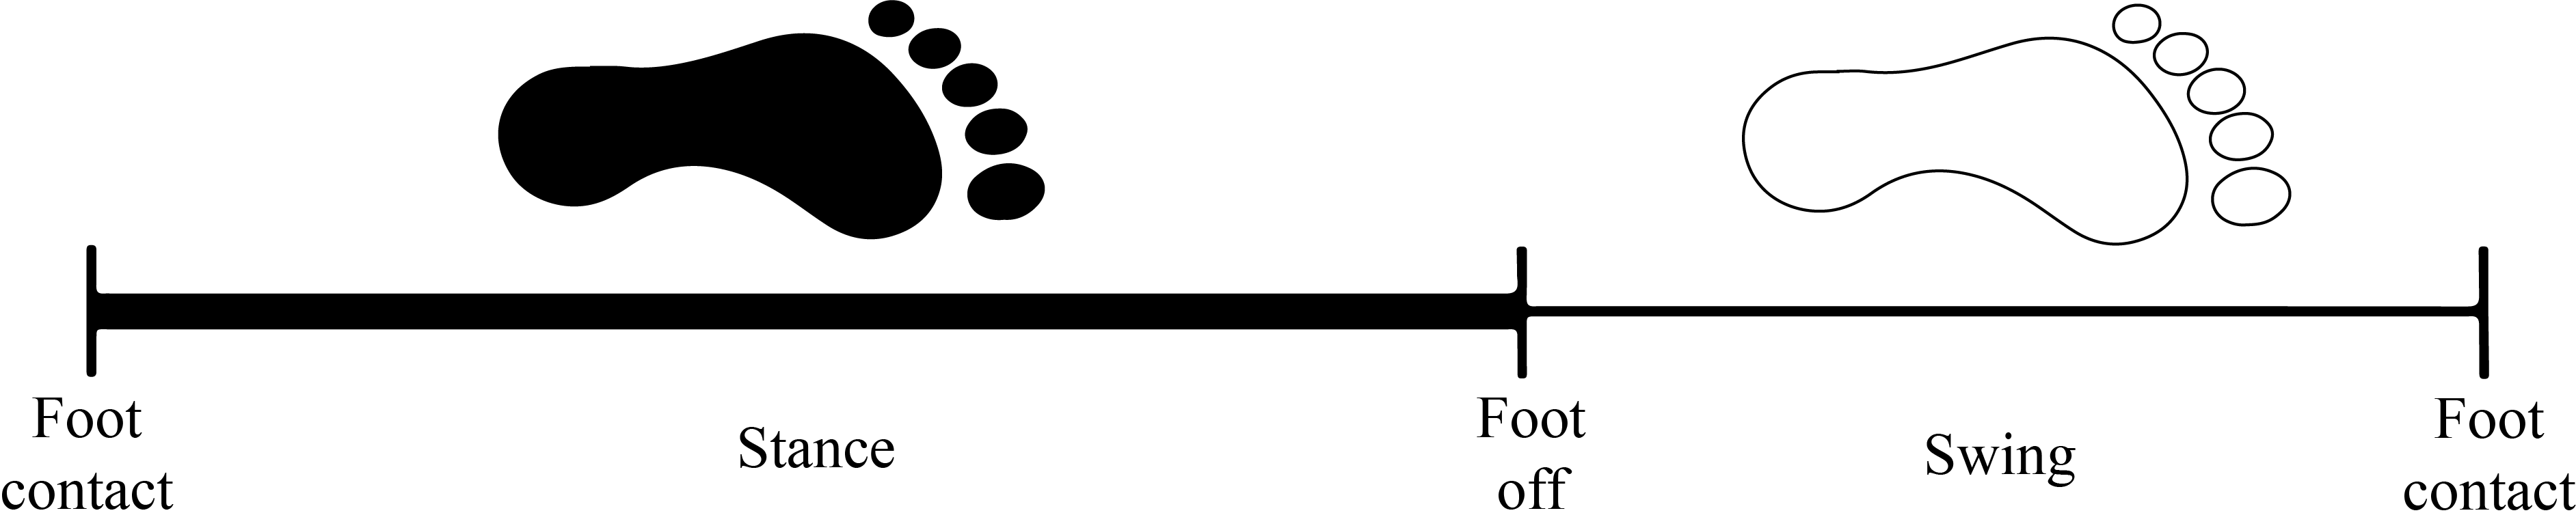
\includegraphics[width=1\textwidth]{gait_phases.png}
%     \caption[One side gait phases]{One side gait phases. Source: edited by author from \cite{Baker2013}.}
%     \label{gait_phases}
% \end{figure}

% The scheme can include the events of both legs, and is divided into first double support (both feet in contact with ground), single support, second double support and swing, as is shown in figure \ref{gait_phases_ds}. Single support and swing are long phases, so a subdivision is a good choice: \textit{early}, \textit{middle} and \textit{late} as can be seen in the figure \cite{Baker2013, Schneck2002}.

% \begin{figure}[b]
%     \centering
%     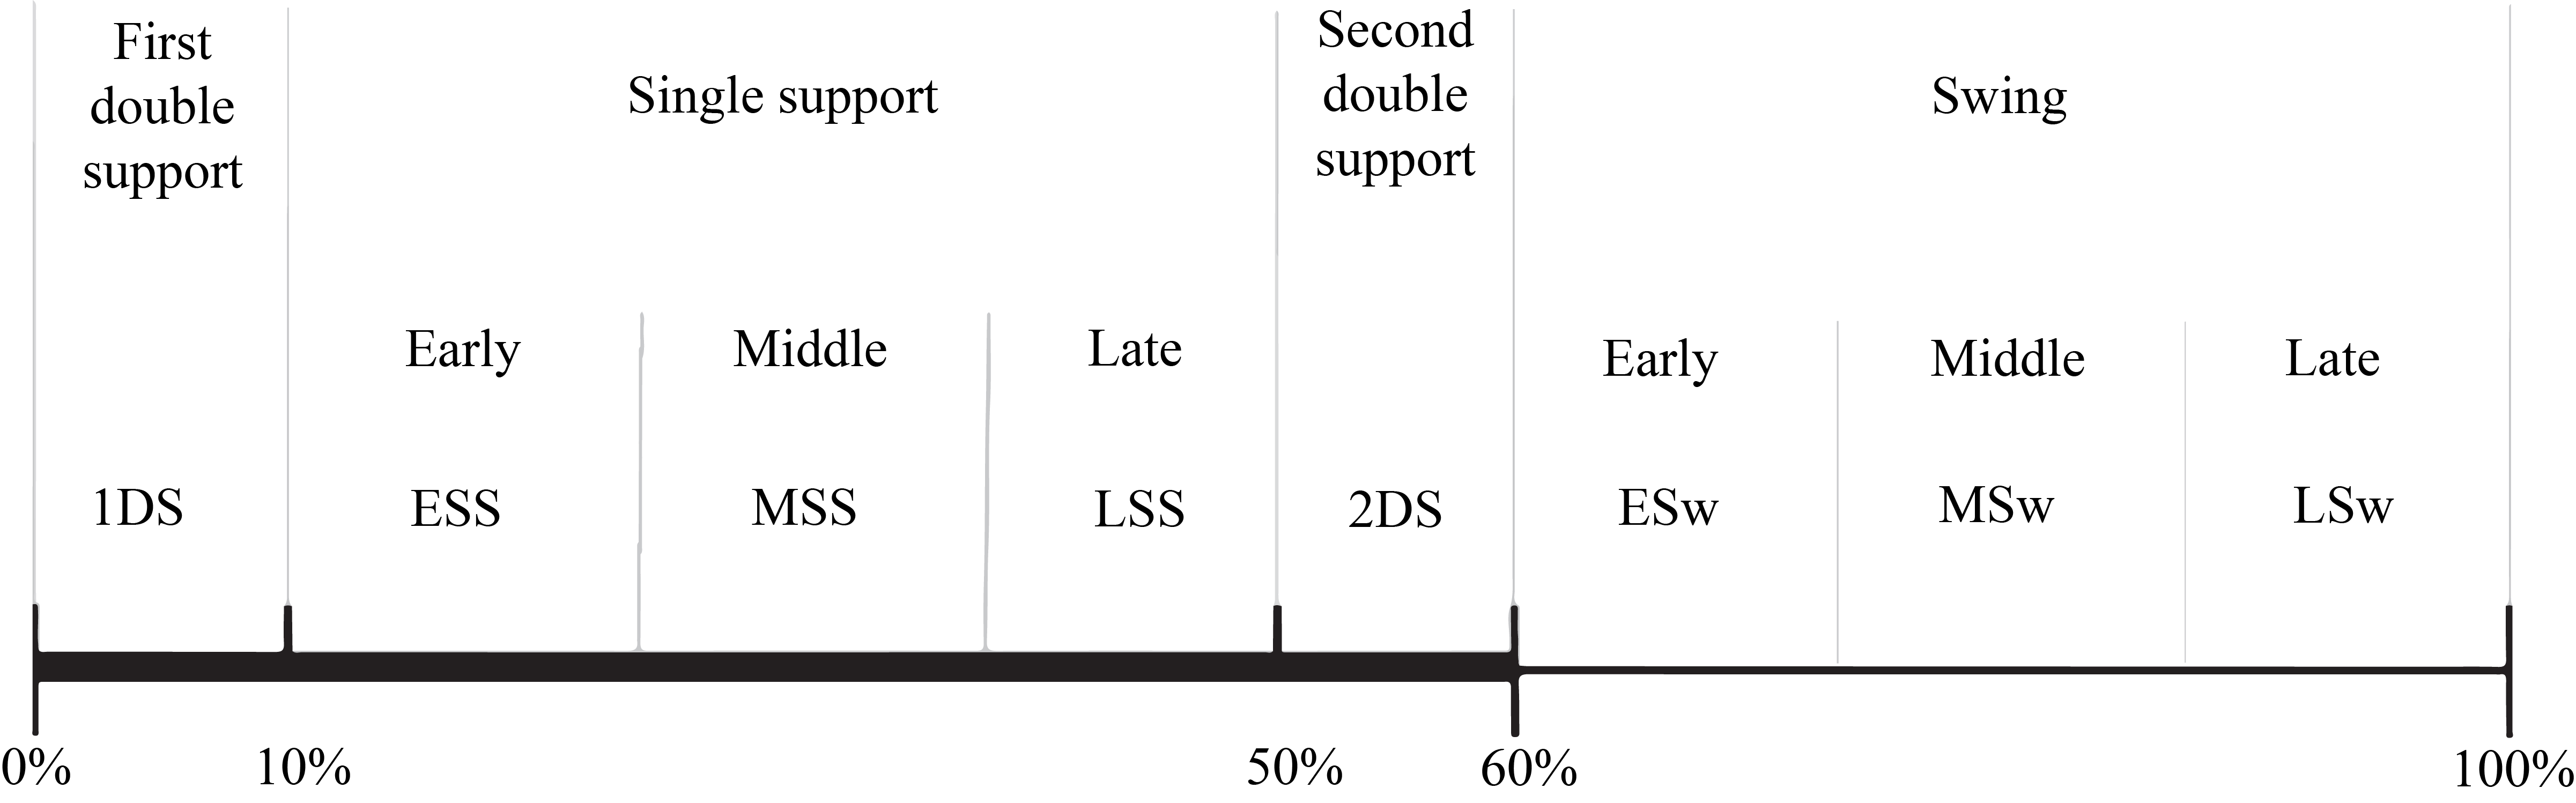
\includegraphics[width=1\textwidth]{gait_phases_ds.png}
%     \caption[Both sides gait phases ]{Both sides gait phases. Source: edited by author from \cite{Baker2013}.}
%     \label{gait_phases_ds}
% \end{figure}